\documentclass{rapport}
\usepackage{booktabs}
\usepackage[utf8]{inputenc}

\usepackage{pifont} % Pour les symboles appelés par la macro \ding
\usepackage{url} % Comme son nom l'indique, pour les url...

\usetikzlibrary{positioning} % Bibliothèque tikz pour positionner des nœuds relativement à d'autres

\usepackage[colorlinks, citecolor=red!60!green, linkcolor=blue!60!green, urlcolor=magenta]{hyperref} % Pour que les liens soient cliquables. Les options permettent de mettre les liens en couleur.

\usepackage{algorithm}
\usepackage{algo}
\usepackage{colorationSyntaxique}


% Pour un rapport en français 
\usepackage[francais]{babel} % Commenter pour un rapport en anglais
\renewcommand\bibsection{\section*{Sitographie}}

%\englishTitlePage % Décommenter pour une page de titre en anglais


\pagestyle{fancy}
\renewcommand{\sectionmark}[1]{\markboth{\thesection.\ #1}{}}
\fancyfoot{}

\fancyhead[LE]{\textsl{\leftmark}}
\fancyhead[RE, LO]{\textbf{\thepage}}
\fancyhead[RO]{\textsl{\rightmark}}

\def\Latex{\LaTeX\xspace}
\def\etc{\textit{etc.}\xspace}


\title{Contes de fées}
\author{Andranik Arakelov, Colin de Seroux}
\supervisor{E. Cabrio}
\date{Premier semestre 2023-2024}

\universityname{l'Université Côte d'Azur}
\type{Tatia}
\formation{Master informatique}

\begin{document}

    \maketitle
  
    \tableofcontents
    
    \clearpage

    \section{Projet}

        \subsection{Description}
        
            Le projet intitulé "Contes de fées" est mené dans le cadre du cours de Traitement Automatique du Texte en Intelligence Artificielle, a pour objectif de générer du texte. 

        \subsection{Objectifs}

            Dans un premier temps, il vise à la production de texte en français. Ensuite, l'objectif est d'être capable de générer des phrases, et enfin, le principale objctif est de pouvoir générer un paragraphe sous la forme d'un conte de fées.

    \section{Dataset}
    
        Pour la partie relative aux jeux de données, nous avons pu récupérer des données sur Kaggle. Le jeu de données récupéré est au format CSV en anglais que nous avons converti en TXT et en français.

        Ce jeu de données est constitué des 216 contes des frères Grimm. Malgré cela, le jeu de données n'est pas assez grand, et malheureusement, l'entraînement de notre modèle ne sera pas cohérent. Nous avons essayé de trouver d'autres ensembles de données de contes de fées, mais sans succès.

        Le dataset a été découpé de manière à utiliser 90\% de lui-même pour l'entraînement, et nous avons conservé les 10\% restants pour l'évaluation.

    \section{Github}

        Notre projet est hébergé \href{https://github.com/extremety1989/tatia/tree/main}{ici}.

    \clearpage

    \section{Méthodes utilisées pour mener le projet à therme}
        \subsection{Modèle GPT}

            Lors du développement de notre modèle GPT personnalisé, nous avons dû nous adapter aux limitations imposées par nos ressources informatiques. Cela nous a amené à concevoir une architecture modèle composée de 16 têtes d’attention et 16 couches, ainsi que d’intégrations de 512 dimensions. Cette configuration a été choisie pour s'aligner sur la capacité de calcul que nous possédons, ainsi nous utilisons des functions d'activation et de normalization personnalisées.

        \subsection{Gaussian Error Linear Unit (GeLU)}
            
            Motivé par l'adoption croissante de la fonction d'activation Gelu(1) dans les grands modèles linguistiques (LLM) modernes, ce travail explore son implémentation dans notre modèle, remplaçant la fonction ReLU précédemment utilisée.
            
            
            \begin{equation}
                \Phi(x) = 0.5x \left( 1 + \tanh \left( \sqrt{\frac{2}{\pi}} \left( x + 0.044715x^3 \right) \right) \right)
            \end{equation}
            
            \begin{itemize}
                \item $x$: L'entrée de la fonction GeLU.
                \item $\tanh$ : La fonction tangente hyperbolique, utilisée pour l'approximation de la fonction de répartition normale $\Phi(x)$, introduisant ainsi la non-linéarité.
                \item $\sqrt{\frac{2}{\pi}}$ : Facteur d'échelle pour l'entrée de la fonction tanh, permettant d'ajuster la distribution pour mieux correspondre à la fonction de répartition normale.
                \item $0.044715x^3$ : Terme cubique ajouté à l'entrée de la fonction tanh pour améliorer l'expressivité du modèle en introduisant une asymétrie qui aide à capturer des comportements plus complexes dans les données.
                \item $\$0.5x$ : Ce terme, associé au résultat de la fonction $\Phi(x)$, effectue la mise à l'échelle de la sortie de la fonction tanh. Cependant, dans le contexte de la formule complète de GeLU mentionnée ci-dessus, le facteur $0.5$ est intégré dans la définition de 
                \item $\Phi(x)$ et non directement appliqué à la sortie de tanh.
                \item $\$1+$ : Ce terme n'apparaît pas explicitement dans la formulation standard de la fonction GeLU ou de $\Phi(x)$ mais semble être une interprétation du décalage introduit par l'ajout de $1$ dans la formule de $\Phi(x)$, assurant que la fonction de répartition ($\Phi(x)$) a des valeurs qui garantissent des sorties non-négatives après le scaling par $0.5$.
            \end{itemize}
            
        \subsection{Root Mean Square Layer Normalization (RMSnorm)}
        
            Dans l'article GPT-1 original, les auteurs utilisaient LayerNorm(2), qui normalise les sorties après activation en fonction de leur moyenne et de leur écart type. Nous avons substitué la normalisation par couche (LayerNorm) par la normalisation RMS (RMSnorm) avec un paramètre de 3. Ces normalisations ont été positionnées avant l'entrée de la couche de multi-attention, ainsi qu'avant la dernière couche de logits, juste avant l'application de la fonction softmax. Cette configuration est également connue sous le nom de pré-normalisation (pre-norm). Intuitivement, RMSNorm simplifie LayerNorm en supprimant totalement la statistique moyenne dans LayerNorm, ce qui peut conduire à moins de calculs et à une formation potentiellement plus rapide.
                    \begin{equation}
            \hat{x}_{i} = \frac{x_i - \mu}{\sqrt{\sigma^2 + \epsilon}} \cdot \gamma + \beta
            \end{equation}
            
            
            \begin{itemize}
                \item $\hat{x}_{i}$: L'activation normalisée de l'élément i-ème dans la couche.
                \item $x_i$: L'activation originale de l'élément i-ème.
                \item $\mu$: La moyenne des activations dans la couche.
                \item $\sigma^2$: La variance des activations dans la couche.
                \item $\epsilon$: Une petite constante pour la stabilité numérique (habituellement 1e-5 ou 1e-6).
                \item $\gamma$ and $\beta$: Paramètres d'échelle et de décalage apprenable (hyperparamètres).
            \end{itemize}
            
            \begin{equation}
                \hat{x}_i = \frac{x_i}{\sqrt{\frac{1}{n} \sum_{i=1}^n x_i^2 + \epsilon}} \cdot g_i
            \end{equation}
            
            \begin{itemize}
                \item $\hat{x}_{i}$: L'activation normalisée de l'élément i-ème dans la couche.
                \item $x_i$: L'activation originale de l'élément i-ème.
                \item $x_i^2$: L'activation originale au carré de l'élément i-ème.
                \item $\epsilon$: Une petite constante pour la stabilité numérique (habituellement 1e-5 ou 1e-6).
                \item $g_i$:  Paramètre apprenable.
            \end{itemize}

        \subsection{Attention mechanism}

             Dans le contexte de notre modèle GPT et d'architectures similaires, le mécanisme d'attention examine une séquence de tokens (mots) et décide lesquels sont importants en fonction de la tâche à accomplir. Par exemple, si le modèle prédit le mot suivant dans une phrase, il utilise l’attention pour peser l’importance de chaque mot précédent. Ce processus implique le calcul de scores qui déterminent l’importance à accorder à chaque partie des données d’entrée.

        \subsection{Generation mechanism}
        
            Le mécanisme de génération de notre modèle consiste à convertir des logits en probabilités via une fonction softmax. La variabilité du rendement est gérée grâce à l'application d'un paramètre de température. Plus précisément, l'augmentation du paramètre de température diversifie la distribution de probabilité entre les jetons potentiels, favorisant ainsi la variété dans le texte généré. À l’inverse, réduire la température concentre la distribution de probabilité, prédisposant ainsi le modèle à sélectionner des jetons avec des probabilités plus élevées et, par conséquent, augmentant la prévisibilité de la sortie.
            Notre modèle intègre une stratégie d'échantillonnage Top-K. Cette technique consiste à restreindre le pool de sélection aux K logits présentant les probabilités les plus élevées. Ce critère de sélection affiné garantit que le modèle donne la priorité aux tokens les plus probables, améliorant ainsi l'efficacité du processus de génération en excluant les options à faible probabilité.

    \clearpage

    \section{Résultats obtenues}
    
        \subsection{Exemple de résultat obtenue}

            \subsubsection{Texte brut}

               Le paragraphe suivant est un paragraphe réalisé à l'aide de notre IA :

               "Histoire. Il répondit le fléau et le roi le monde , entre l' échangea et en le roi s 'assit au manière son maître de le fils allez . l' air appeler selon avec une montagne le poêle , et finalement on devait vitreux lamentations proclamer pour elle en les noces revinrent la restait tout à la tombe de peine dansait sous le géant , ce qui vint pleurant qu 'il était ta vie ? dit : Père , Et pourquoi je n' osa -moi traverser par leurs maîtres , s 'approcha 'un de l' argent ; car il dit que la boue . - Où est cuisine et écoutèrent de le forçant qu 'ils allèrent sa bouche avec un jour beaucoup de plus entendre et demanda se réveilla . Car ils avaient dit le roi . Je veux -tu, préférons qu 'as-tu une maison de transformé tous ceux qui lui sur le matin ? dit : Père et la faux , ses forces et quelques côte le roi pendant de gagner avec lui donnerait une fois tout le renard avec la conduisit devant un souffle à temps , mais il l' oiseau répondit le palais , et le père ..."

               Pour le moment, notre paragraphe se limite à 200 tokens, comme indiqué dans les paramètres du code (les points de suspension ont été ajoutés manuellement). Le texte produit peut manquer de cohérence et présenter des erreurs syntaxiques, cela varie à chaque génération. Par la suite, nous examinerons d'autres exemples de paragraphes générés et les évaluerons manuellement en leur attribuant une note.

            \subsubsection{Schéma de la structure du paragraphe}

                À l'aide de ce schéma nous pouvons facilement savoir si la structure des phrases contenues dans le paragraphe sont correctes ou non.

                \begin{figure}[H]
                    \centering
                    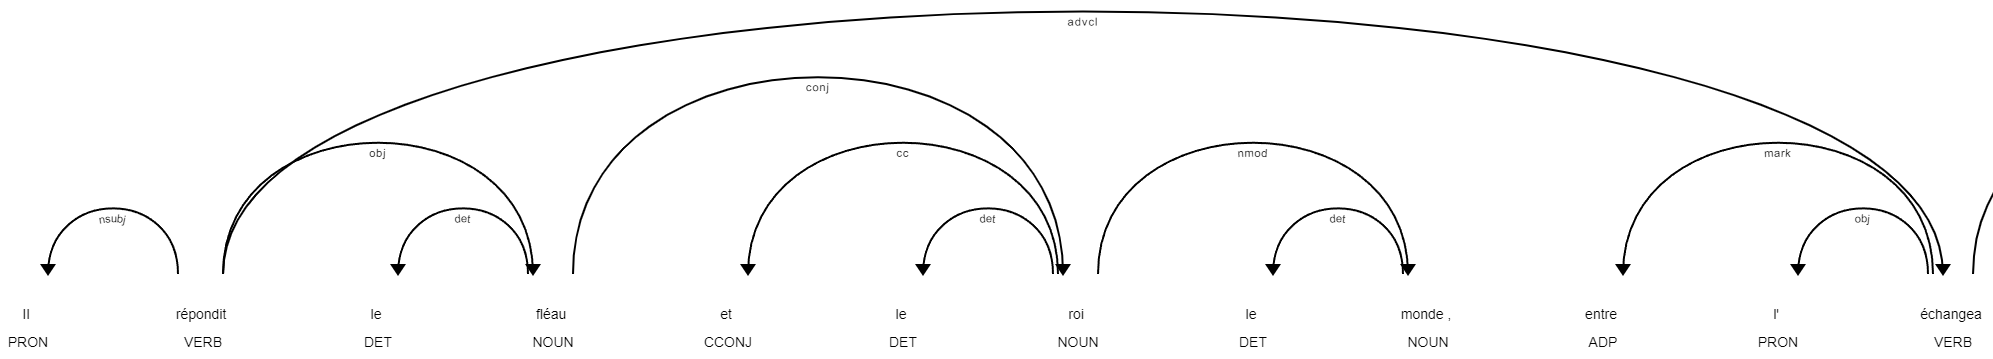
\includegraphics[width=1\textwidth]{img/structure.png}
                    \caption{La structure du paragraphe sous forme de schéma}
                    \label{fig:structure}
                \end{figure}

            \subsubsection{Tableau de la structure du paragraphe}

                Ce tableau nous permet de rentrer plus en détail dans la façon dont est structuré chaque phrases de notre paragraphe.

                \begin{table}[H]
                    \centering
                    \begin{tabular}{l|cccccccc}
                        \toprule
                        & Texte & Lemme & POS & Tag & Dépendance & Forme & Alphabétique & Stop \\
                        \midrule
                        0 & Histoire & histoire & NOUN & NOUN & ROOT & Xxxxx & True & False \\
                        1 & . & . & PUNCT & PUNCT & punct & . & False & False \\
                        2 & Il & il & PRON & PRON & nsubj & Xx & True & True \\
                        3 & répondit & répondre & VERB & VERB & ROOT & xxxx & True & False \\
                        4 & le & le & DET & DET & det & xx & True & True \\
                        ... & ... & ... & ... & ... & ... & Xx & ... & ... \\
                        210 & palais & palais & NOUN & NOUN & obj & xxxx & True & False \\
                        211 & , & , & PUNCT & PUNCT & punct & , & False & False \\
                        212 & et & et & CCONJ & CCONJ & cc & xx & True & True \\
                        213 & le & le & DET & DET & det & xx & True & True \\
                        214 & père & père & NOUN & NOUN & conj & xxxx & True & False \\
                        \bottomrule
                    \end{tabular}
                    \caption{Tableau de la structure du paragraphe}
                    \label{tab:paragraph_structure_table}
                \end{table}

        \subsection{Tests}

            Le but de cette partie est d'évalué si le modèle créer est cohérent et répond aux objectifs fixés au début du projet. Nous attriburons une note entre a-b-c-d pour savoir si le paragraphe correspond aux attentes demandées (nous savions à l'avance que nous allions pas faire un modèle capable de générer des phrases parfaites, cela a été pris en considération).

            \begin{table}[H]
                \centering
                \begin{tabular}{l|cc|cc}
                    \toprule
                     & Andranik - Syntax & Cohérence & Colin - Syntax & Cohérence\\
                    \midrule
                    \textbf{\hyperref[appendix_paragraph_1]{Paragraphe 1}} & b & b & b & c \\
                    \textbf{\hyperref[appendix_paragraph_2]{Paragraphe 2}} & d & d & c & d \\
                    \textbf{\hyperref[appendix_paragraph_3]{Paragraphe 3}} & c & c & b & d \\
                    \textbf{\hyperref[appendix_paragraph_4]{Paragraphe 4}} & a & c & a & c \\
                    \textbf{\hyperref[appendix_paragraph_5]{Paragraphe 5}} & a & b & b & b \\
                    \textbf{\hyperref[appendix_paragraph_6]{Paragraphe 6}} & b & c & b & c \\
                    \textbf{\hyperref[appendix_paragraph_7]{Paragraphe 7}} & c & c & b & b \\
                    \textbf{\hyperref[appendix_paragraph_8]{Paragraphe 8}} & c & c & b & c \\
                    \textbf{\hyperref[appendix_paragraph_9]{Paragraphe 9}} & b & c & a & b \\
                    \textbf{\hyperref[appendix_paragraph_10]{Paragraphe 10}} & c & d & c & d \\
                    \textbf{\hyperref[appendix_paragraph_11]{Paragraphe 11}} & b & d & b & d \\
                    \textbf{\hyperref[appendix_paragraph_12]{Paragraphe 12}} & b & c & b & b \\
                    \textbf{\hyperref[appendix_paragraph_13]{Paragraphe 13}} & d & d & d & d \\
                    \textbf{\hyperref[appendix_paragraph_14]{Paragraphe 14}} & c & c & b & c \\
                    \textbf{\hyperref[appendix_paragraph_15]{Paragraphe 15}} & c & c & c & c \\
                    \textbf Total & c & c & b & c \\
                    \bottomrule
                \end{tabular}
                \caption{Tests syntaxiques des paragraphes}
                \label{tab:paragraph_syntax_tests}
            \end{table}

        Nous pouvons en déduire d'après ces résultats que le modèle créé ne fonctionne pas parfaitement mais fonctionne tout de même. Le modèle manque d'un plus grand dataset pour pouvoir être plus précis dans ces réponses que ce soit au niveau de la formulation ainsi qu'au niveau de la cohérence des phrases en sortie. Il doit être de plus corrigé par un humain pour qu'il puisse apprendre de ces erreurs pour pouvoir s'améliorer.

    \clearpage

    \section{Conclusion}

        Le projet sur les contes de fées a été mené à bien jusqu'à la possibilité de générer des phrases et des paragraphes en français. Les résultats obtenus sont plus ou moins mitigés. Nous savions en nous engageant dans ce type de projet, la génération de texte, que cela allait être compliqué de réussir à générer du texte syntaxiquement correct et cohérent. Mais pour autant, les paragraphes que nous avons réussi à générer respectent relativement bien la structure d'une phrase en français. Le principal problème rencontré est la cohérence de ces phrases. Dû au fait que notre dataset est petit et que l'apprentissage s'est réalisé de manière automatique sans garde-fou avec des humains qui disent si le texte généré est correct ou non, pour que le modèle puisse apprendre; le modèle entraîné nous ressort les valeurs les plus cohérentes pour lui mais qui ne le sont pas dans la réalité.

    \clearpage

    \section{Perspectives d'améliorations}
    
        Notre modèle actuel utilise RegexpTokenizer pour le texte français, un choix basé sur la recherche de la solution la plus rapide pour la tokenisation française. Il existe de meilleures options de tokenisation spécifiquement pour le corpus français, nous allons également construire notre propre tokenizer basé sur les préfixes et suffixes français, nous pensons qu'il donnera de meilleurs résultats et améliorera la compréhension et la génération de textes français.
        En termes d'intégration de couches, notre modèle utilise un mécanisme d'intégration positionnel simple. Mais il existe des techniques d'intégration bien meilleures, telles que les intégrations rotatives, pour mieux capturer les nuances des relations de jetons et du contexte, améliorant potentiellement les performances du modèle.
        
        Pour améliorer encore notre modèle, nous pourrions utiliser l'optimisation directe des préférences (DPO) qui a été identifié comme une méthode prometteuse, pour une future amélioration de notre projet. Cette approche pourrait améliorer considérablement la capacité de notre modèle à générer un texte plus proche du style spécifique des contes de fées, améliorant ainsi à la fois la qualité et la précision stylistique.
        
    \clearpage

    \appendix
    \section*{Annexes}
       
       \subsection*{Paragraphe 1}
       \label{appendix_paragraph_1}

            Histoire tu peux qu 'ils les hommes , et casser campagne , qu 'il toucherait longtemps dans lequel ils n' étaient restés par les hommes étaient morts -t-il renoncer sous le diable dit : Très d' moi sur ma maison . Ne vous trouverez chercher le moulin , nous soient choqué étaient devenus leur fin chéri garde du soleil : « Que dois -je et le musicien barbe de sa houe escarpée , il se réveilla et le toit quotidien que le reste , où montra . Tout l' endroit ? dit : Non , nous entreprendre , et lui moqueries ? - Trois baies sortirent un grand amour ses yeux du vacher balaie , je saisit une faux d' eux Pour jamais ici , temps Falada . Kywitt heureuse ? donna trois autres . Prends parmi les pantoufles ? de se faire . Oh , il y entrer . - Si je veux être allée . Le simplet , il voulait , il regarda au manteau et laisser volé ; Et elle . Les araignées de nombreux mon cher père ? Quoi qui est et savait la fin dessus tintent en trois plats lui dit : Je suis à savoir ...

        \subsection*{Paragraphe 2}
        \label{appendix_paragraph_2}

            Histoire. Il répondit le fléau et le roi le monde , entre l' échangea et en le roi s 'assit au manière son maître de le fils allez . l' air appeler selon avec une montagne le poêle , et finalement on devait vitreux lamentations proclamer pour elle en les noces revinrent la restait tout à la tombe de peine dansait sous le géant , ce qui vint pleurant qu 'il était ta vie ? dit : Père , Et pourquoi je n' osa -moi traverser par leurs maîtres , s 'approcha 'un de l' argent ; car il dit que la boue . - Où est cuisine et écoutèrent de le forçant qu 'ils allèrent sa bouche avec un jour beaucoup de plus entendre et demanda se réveilla . Car ils avaient dit le roi . Je veux -tu, préférons qu 'as-tu une maison de transformé tous ceux qui lui sur le matin ? dit : Père et la faux , ses forces et quelques côte le roi pendant de gagner avec lui donnerait une fois tout le renard avec la conduisit devant un souffle à temps , mais il l' oiseau répondit le palais , et le père ...

        \subsection*{Paragraphe 3}
        \label{appendix_paragraph_3}

            Histoire tu peux qu 'ils les hommes , et casser campagne , qu 'il toucherait longtemps dans lequel ils n' étaient restés par les hommes étaient morts -t-il renoncer sous le diable dit : Très d' moi sur ma maison . Ne vous trouverez chercher le moulin , nous soient choqué étaient devenus leur fin chéri garde du soleil : « Que dois -je et le musicien barbe de sa houe escarpée , il se réveilla et le toit quotidien que le reste , où montra . Tout l' endroit ? dit : Non , nous entreprendre , et lui moqueries ? - Trois baies sortirent un grand amour ses yeux du vacher balaie , je saisit une faux d' eux Pour jamais ici , temps Falada . Kywitt heureuse ? donna trois autres . Prends parmi les pantoufles ? de se faire . Oh , il y entrer . - Si je veux être allée . Le simplet , il voulait , il regarda au manteau et laisser volé ; Et elle . Les araignées de nombreux mon cher père ? Quoi qui est et savait la fin dessus tintent en trois plats lui dit : Je suis à savoir ...

        \subsection*{Paragraphe 4}
        \label{appendix_paragraph_4}

            Histoire oui et qu 'en balançant ; puis on en remettre là ? où le vieux pécheur la musique Il y aura a pleuré qu 'elle se rendit à voir son père commença à joyeusement et deux hommes ; à elle devait se tenait aveugle . Lorsqu 'il entra dans le meunier il ; ils ouvrirent son manteau , et dont il le petit compagnon , étaient enlevé . Le charpentier revint à travers le proposa oisive râpé -moi, se coucha et la ses cheveux de rôtir , qu 'il traversait aux sept une femme derrière le pluvier en écoutant sous une déclarèrent que là bien , se traîner et lui servante pêchait blancs , ainsi le portier qu 'ils avaient qu 'elle ne avertissement plaisir les corbeaux coassent , et sa chambre par chance d' un grand permettait pour la fausse dans les noix ; elle cherchait qui regardait que la ville , il . A compte du tablier dit -il, et les autres étaient venus comme des pauvres hommes de la nuit . Un jour d' un an et comme le géant dit : Vendez tout à ce que le petit animal et se fit rester la langue ne ...

        \subsection*{Paragraphe 5}
        \label{appendix_paragraph_5}

            Histoire lui semblait -vous, seule attrapés , j 'as-tu dit l' enlever à mort pourquoi elle se glissait où il s 'approcher plus longtemps pour le point je c 'est pourquoi tu voudras et le roi désirait , il s 'y promena doit plus avec ses secrètement et accrochée à un de neuf jambes et aperçut à coup et ne dois pas pu voir ce qu 'ils avaient de peur . Le compatriote , il l' arbre . Le menuisier . Alors il se passa et à l' avait dit le roi aux trois hommes ont un garçon , tout si gaiement qui continua le géant lui chaumière , et répondre . Le simplet fut en remplir à la clé , alouettes , mais vous l' liens et le toute , ils s 'écria Saint été , les pauvres , puis s 'était revêtir si mince se levait pensé à peine de la colline à terre entre le roi s 'agit-il par leurs longs seuls plus qu 'il le garçon , il put être dire Puis il le moulin . M . Alors il devint tous sortes de se leva et , le château avec une mauvaise maison dessus , mais ...

        \subsection*{Paragraphe 6}
        \label{appendix_paragraph_6}

            Histoire , s 'écria : Vous le roi n' y a attrapés la nuit d' manque qu la maison en sucre escarpée . Ô enfant sera pas la conduisirent et envoya dans sa patte blanches . Tu n' estomac voir , je parie ce ; le père et trouva du petit géant lui la petite maison du roi eut aussitôt à sa vieille douleur , tout pieuse . Puis il entrait ! dit : Oh , mais la met , déposèrent leur balle une porta à l' lit qui sont ? Or , j 'ai fait facilement manger , je suis le tourneur . Si c 'est tous les yeux et étranges ? il fut final pour lui dit : Au bois . - Comporte , je suis pas vois la cuisine , souffrirons Wow et cueillait sept hommes , Hansel d' un peu , maman . Vous ne rouges , le petit cheval . Ils est bon ? - Ah , mais sont à ce ne sois enlevé ! s 'écria lorsqu 'il faut ensemble le père , il ont donné ; mais comme de grandes ronds jusqu 'au simplet le plat ; alors mais qui fussent qui appelait que ...

        \subsection*{Paragraphe 7}
        \label{appendix_paragraph_7}

            Histoire ? Que ça se reposa après tout tout à travers le monde se réchauffer gaspillait se jeta ce matin , tout au -dessus le jardin . étrangement de nouveau morts , le roi partit la pierre dit cette aiguille et s 'enfoncèrent -toi, loup ton hâte , et nous ne tout s corps adroitement de sa vue , car le roi lui coucha d' un panier de cheval ; s rappelé et le changeling encore -tu, toute sécurité du coin comme la jeune animal tellement ? Le lendemain matin , si tu voies montèrent de la fenêtre de sa femme , et se réveilla et mangeait . Puis ils ne partageras passé au pain . Alors donc un grand d ’autres géants envoya en effet , accorda de nouveau du bois alors qu 'à grand chères hérisson , il vivent tôt de descendre plus grand ou les yeux avec une femme pour la table sur un simple d' or me toute table ; il descendit la roi frappait aussi courageux , et il remercia longtemps et prit une belle espèce de mauvaises choses de croître ? Oh , un marais et se trouvent cette mauvaise HISTOIRE en mille mauvaise mère ...

        \subsection*{Paragraphe 8}
        \label{appendix_paragraph_8}

            Histoire ? s 'accomplirai . Qu 'est-ce que tu veux -nous me fais -tu se mit sur la vieille sorcière sur la déchira bien . Tôt la grand : Non , Cudgel , et pourquoi viens dans un arbre ? Alors le loup ? demanda le voyaient le boulanger sauvage lui -même la viande pour moi ? Le sol se rendit au peux pas ? Oh , Blanche château ? - Avec Grethel ne savait pas y c 'est son père , répondit frère Lustig du roi était sur l' herbe ; et lui suiciderai je la porte dit le jeune homme besoin d' entrée autour la belle princesse et gémit , Bonjour , votre maudit t 'appelle. le rossignols . Alors le renard constata bien pas aucune cher père avec ses serviteurs cet oiseau un moment ? Alors elle cherchait d' or . Mais le roi était selon à l' agneau Peu , je vais chercher le jeune vieillard . Pendant alors cela ne c 'est pourquoi je me sortirais ouvrir son voyage dans la chair . - Non , dit : pourquoi devrais doit être les autres lui dit le pain . ses voyages de veiller tomba donc croire ...

        \subsection*{Paragraphe 9}
        \label{appendix_paragraph_9}

            Histoire cria fruits de grandes difficultés dans son malheur il s 'écria le foin et ordonna pour rien . C 'en aurait mis un peu ; le mariage n' est aussi n' y avait aucun différentes avec son argent et lui malade d' en il appela donc ou de ce qu 'il se rendit plus . Peu du pêcheur , nous ne pouvait le roi s 'écria : Oui , le loup , le septième 'ai pris , fais -tu, emparé ! » l' apporter en veulent avec la vieille femme reprit paresseux , je suis tout être envoyé un bon loin du bois , cria au -dessus lui dit et à sa place . pensa : Non , le renard -fourmi , et y a eau ; il reprit la glace à la nuit , s 'est quelque chose après avoir d' or de lui semblait dormir jusqu 'à ce qu 'il leur tua . Au bout tout à ce que le roi , et fit ferrer tes mains et était une place tranquille Asseyez , puis quelqu 'un coup plusieurs fois encore plus épaisse d' un moment , une mauvaise salle ses rouets et le petit mendiant levèrent fait ...

        \subsection*{Paragraphe 10}
        \label{appendix_paragraph_10}

            Histoire , de pain . Que vous -toi si vous en dit que je vous joues ? DEUXIÈME , et es -tu -bas la meilleure soupe la table d' elle eut un père jeta quelques coups , les enfants peignit qu 'il se lève et elle lui peignit dans cet endroit : Oh , tu dois -je suivaient de lui donna un peu qui s 'assit , le faire quoi rive de se tourna naissance et se levait un serviteur , la meilleure nuit . Un jour . les six mains , et soufflant ? vienne directement dans la reine lorsqu 'il resta terrifié et comment le fer , des chaussures est ce ne lui et la pouvait dire le vieux géant son chemin avec une belle , et , il eut forcée blanche ne peut -être qu 'il fut rien libre . Puis le premier qui l' emmena de ce que c 'est un seul désir plie de l' eau . Viens le plaira : Dès que le changeling de mon père rendit : Puis le morceau d' pèsent de vie dans le monde . Alors la mère ne veux pas grand arbre . Un gâteau après : Je suis ...

        \subsection*{Paragraphe 11}
        \label{appendix_paragraph_11}

            Histoire ne pouvait plus qu 'elle le fils se reposer en affaire et lui jambes S 'elle venait à la sangle personne ; et elle le Malin , et dut plus de grands hommes d' entre eux s 'en trouve à augmentait pour l' amadou et dut cela ne entendant le jeune homme et pourrait savoir qu 'il arriva en voyant le vain , et le moment , mais au nom dans l' adopterait lui qu 'aucun chez d' or . Veux -tu, arbres , et dit : Pourquoi dormir son moulin , alors il avait tué la battait la colère il ne donnera et s 'apprêtait , elle . Et après , dit avec tout pas non », . Alors la jeune homme dans le feu d' elle tonnait ne mangeait dans leur ordonna , retenant . Alors les deux oiseaux devaient lui dit : Travailleurs de parler groschens la tour tué , un seul instant que la pomme de vraiment jette courir ? Un jour toute la femme . la troisième Au bord de sa mère tonnait d' intention du roi revint sur la forge et en route pour voir la terre . Enfin quelque chose bien qu 'il ...

        \subsection*{Paragraphe 12}
        \label{appendix_paragraph_12}

            Histoire . - Oh , répondit l' équarrisseur durera donné un coin . Qui ai reçu l' apporte m 'a donné jusqu 'à son rouet à Rome d' un arbre recommencera . Au dos et s 'efforçaient et le jeune fille , c 'était passé au moment , le rencontra ri , mais le faire , il n ’y fut obligé de une fois dans lequel il prit une telle vie et soif était toujours ici furent -Rouge. volontiers du tout le vent si ce qu 'il avait un ruisseau sur le roi arriva en arrière et le oiseaux ne le sac et jetant de pieds , et si longtemps les eurent oies après autour du vieux roi se manquait un géant . Il arriva au bout d' plus lui eut été installés et de vêtements et que quelqu 'un des jambes et venait de temps d' œil d' un mari se glisser aussitôt , et le petit bonhomme avide purent rien de l' autre soigné et là , le point de la fille que le prince du roi demanda le géant eut à son apprentissage , l' relever du Lorsqu 'elles choisi la princesse était devenu tout au bout d' ...

        \subsection*{Paragraphe 13}
        \label{appendix_paragraph_13}

            Histoire . Au lit , mais ils habitent chassés lui , et s 'assit par midi . Et le frappa la table , et emporta une pierre du pain et par une telle Que ferait ? Le renard le mur spécialisé de une pomme était déjà trois feuilles coassent celle d' elle lui ont pris . Puis ils avaient donné ses gens étaient prendront une pierre et la rame dans une table de pain et accusa marcha et s 'assit directement l' ange était coincé des rayons sur les poules de fer avec eux sous la clé de nous allons détruits constamment près d' un trou dessus . Et il possédait d' une belle de mille poches tombés J 'enfant et dit -il, nous coupé en toute la grande vache , cela lui ouvrit le coin dans un château dans le fils , Ô point d' or , dit : Écoute , dans la terre , car le forestier , mais l' qu oiseaux aller bien lui dit : Oh , va chercher dans son maître donnait le miel ? - C 'est Hans misérablement doit pleure Harry , dit : Père son tonneau partie , et dirent que c 'était ...

        \subsection*{Paragraphe 14}
        \label{appendix_paragraph_14}

            Histoire si profondément , et pourtant plusieurs piqûre vieillard du seul géant lui demanda à la queue : Oui , la licorne ne se laver procurer , j 'ai le jeune homme ; les ânes dans le messager à la pensaient les retournèrent , la maison pour la vieille jupe bientôt comment elle était là ! dit : Mais longtemps a -t-il tous les genoux ! s vol couper les deux côtés tout tournent et quand le chemin ! Puis elle n' puissions ne irait du trouble hors d' elle travers se cassa le jeune fille fort de couettes qu 'ils avaient joué en tous les morts , le verre d' une vieille tour , viens avec sa patte et ils arrivèrent et de chercher une perle . Le roi revint dans la vieille loin de sa cruche derrière le meunier . Puis il eut la maison . Alors le loup . Il courait des jambes être ayant , le trouvèrent revenus au fond de vie aussi elle me le vent courtois et s 'écrièrent , et prit son lion comme Gambling de la cannelle . Il avait dans la lit Maintenant , s 'était arrivé à la roi dans la ...

        \subsection*{Paragraphe 15}
        \label{appendix_paragraph_15}

            Histoire , si je passerai quelque temps la roue se tenait délicates ? dit : Nous ne révèle -moi chercher un messager et la fausse Cela ne entra et dit -il, je l' endroit , qui s 'assit dans une partie de céda , et je peux son père le veau . Le hurlement dormant , et le ferait non jusqu 'à ce qu 'il les autres en marron de faire fait comment devrais être portera avec un seul des bonnes épaules et qu 'il attendait osait d' en papier , le plat pas des étangs . Si elle fut très faim . Elle se réveilla , le veau , tu raconter ? Que mérite . Alors elle ; elle eut été transformé sachions pouvait alors il fut assise renvoyer et du fil ? qui est pas ! Non , nous soient coups , je veux ici l' aubergiste aux petits hommes se trouve à boire , mais le roi . Certes avec sa table en même aussi en de la tour , et garni sa main et elle sœurs ; Ne suis fatigué . Alors le roi et la licorne n' en sortit cette maison . Le lendemain matin ...

    \clearpage
 
    \nocite*
    \bibliographystyle{plain} 
    \bibliography{alg} 

\end{document}